%************************************************
\chapter{Methods}\label{ch:methods}
%************************************************
This chapter explains the relevant methods and procedures for answering the sub-questions that are proposed in the introduction (\autoref{ch:introduction}). It is divided into several sections, whereas every section answers a specific sub research question.

\section{Collecting the utilization} \label{sec:collect_utilization}
In the sections below, an architecture for collecting the utilization of a Cloud Computing System will be discussed. This answers Q2, which is the following research question:

\begin{quote}
	\textbf{Q2: }\textit{How can the utilization of a Cloud application be monitored in an effective manner?}\\
\end{quote}

...
\todo{I want to answer this question by explaining the architecture, as well as the p2p communication system}

\section{Estimating the cost} \label{sec:cost}
In the sections below, the cost for hosting a Cloud Computing system will be discussed. To rephrase, the research question that will be answered is:

\begin{quote}
	\textbf{Q3: }\textit{What is an effective approach for computing the waste of a Cloud application?}\\
\end{quote}

...
\todo{I want to answer this question by explaining that the price of a VM can be estimated by a simple formula, for which the data is based on GCE. Additionally, I want to do some research that this price is more or less equivalent accross multiple Cloud Providers}


\section{Computing the waste distribution} \label{sec:waste_into}
In the sections below, the waste computation will be explained, as well as the decision that have been made that are relevant for computing the waste, given the utlization values for a given host. To rephrase, the research question that will be answered is:

\begin{quote}
\textbf{Q4: }\textit{What is an effective approach for computing the waste of a Cloud application?}\\
\end{quote}

\noindent
This question can be considered as a mathematical question, as it consists of a fixed set of input variables, and results in a fixed set of output variables. In order to answer this question it is therefore important to determine the properties of the waste distribution before. The next section comes up with three strategies for computing the waste distribution, that all meet the requirements of the properties below. The last section tries to find the optimal approach, by evaluating the approaches against several properties.

\section{Properties of the waste distribution}
There are several ways in which the utilization values can be used to compute the waste. In this research, the following three properties are used for finding an optimal waste distribution:
\begin{enumerate}
    \item \textbf{$\sum_{i=1}^n w_i = 1 - \sum_{i=1}^n u_i $}: The sum of the elements of the waste and the sum of the elements of the utilization values should sum up to 1, as it implies that a resource is either used (this is $u$) or being wasted (this is $w$).
    \item \textbf{$w_i \geq 0$} for $1 \leq i \leq n$: The waste of every certain container is non negative. Thus, it is impossible for a container to have a negative waste. As the waste distribution is used for computing the amount of money to be wasted, this would imply that money is being earned, while running a certain container.
    \item \textbf{$\max w_i \Rightarrow \min u_i$}: The container that utilizes the most resources, should be responsible for wasting the least amount of resources. This property implies that the order of containers from lowest utilization to highest utilization is the same as the order of containers from highest waste to lowest waste. 
    \item \textbf{$w_i = w_j \iff u_i = u_j$}: If two containers utilizes the same amount of resources, than they should also waste the same amount of resources. The opposite should also hold. If two containers utilizes both a different amount of resources, than it should also have a different amount of waste.
\end{enumerate}

The following section contains several different approaches for computing the waste distribution. In the section that follows this, the approaches are evaluated against the properties above.

\section{Approaches for computing the waste distribution} \label{sec:approaches}
In this section, the following three waste distributions will be evaluated: equal distribution, linear inverse distribution and proportional inverse distribution. They are all described in a different subsection below.

\subsection{Equal distribution} \label{sec:equal}
Using an equal distribution, the waste is the same for every container on a certain host, i.e. $w_1 = w_2 = \dots = w_n$. The idea behind this approach is that a set of containers together wastes the same part of the host and therefore the waste should be distributed over every container in a fair manner. This approach can be computed by the following formula:
\begin{equation}
w_i = \frac{1 - \sum_{i=1}^n u_i}{n}
\end{equation}

\subsection{Linear inverse distribution} \label{sec:linear}
This distribution computes a higher waste for a container that utilizes less, and can be computed by the following formula:
\begin{equation} \label{eq:linear}
w_i = \frac{1}{n} - u_i
\end{equation}
However, it is easy to see that \autoref{eq:linear} returns a negative value if $u_i > \frac{1}{n}$ (contradicts property 2). Therefore, this formula can be replaced by the following formula:
\begin{equation}\label{eq:heuristic}
w_i = \begin{cases}
\frac{1}{n} - u_i & \text{if } u_i \leq \frac{1}{n}\\
0                 & \text{otherwise}
\end{cases}
\end{equation}
This yields another problem, as it is not guaranteed that property 1 holds. In fact, property 1 will fail, if there exists a $j$ for which $u_j > \frac{1}{n}$ (the function returns the \textit{otherwise}-case). Therefore, a simple formula can be used to restore property 1. Note that $u = \sum_{i=1}^n u_i$ and $w = \sum_{i=1}^n w_i$ and needs to be computed before the first $w_i$ is updated.
\begin{equation} \label{eq:update}
    w_i \leftarrow w_i * \frac{1-u}{w}
\end{equation}
An example for $n = 2$ can be the following distribution $u_1 = 0.6$ and $u_2 = 0.3$. After \autoref{eq:heuristic}, the following values are found $w_1 = 0$ and $w_2 = 0.2$. However, since property 1 doesn't hold, $w_2$ is updated to $0.1$. The entire algorithm for this approach is formulated in Algorithm \ref{alg:linear}.

\begin{algorithm}
\caption{Compute the waste based on the linear inverse distribution}\label{alg:linear}
\begin{algorithmic}[1]
\Procedure{computeWaste}{$u_1, u_2, \dots, u_n$}
\For{$i \gets 1 \dots n$}
\State $w_i\gets \max(\frac{1}{n} - u_i,~0)$
\EndFor
\State $u\gets \sum_{i=1}^n u_i$
\State $w\gets \sum_{i=1}^n w_i$
\If{$u+w \neq 1}$
  \For{$i \gets 1 \dots n$}
\State $w_i\gets w_i * \frac{1-u}{w}$
\EndFor
\EndIf
\State \textbf{return} $w_1, w_2, ..., w_n$
\EndProcedure
\end{algorithmic}
\end{algorithm}

    
\subsection{Proportional inverse distribution} \label{sec:proportional}
This distribution uses the idea that the product of the utilization and the waste distribution should be constant for every container. 
The formula is therefore: $w_i * u_i = c$ for an unknown value of $c$. This implies that if a certain container utilizes a high amount of resources, its corresponding waste must be a low number.
The $c$-value is constant across all containers on a specific host, which leads to the general formula: 
\begin{equation} \label{eq:constant}
    w_1 * u_1 = w_2 * u_2 = \dots = w_n * u_n
\end{equation}
However, in case of $n = 1$, there is no equation possible. In this case, the waste can directly be computed using property 1, and thus $w_1 = w = 1 - u_1$.

In general (for $n \geq 2$), \autoref{eq:constant} results in $n-1$ unique equations. However, this set of equations cannot be solved, as there are $n$ variables unknown ($w_1$ to $w_n$). But property 1 can be used to generate $n$ unique equations. For example, for $n=3$ the following equations needs to be solved:
\begin{equation}\label{eq:linear3}
    \begin{split}
        w_1 & u_1 - w_2 * u_2 &= 0 \\
        w_1 & u_1 - w_3 * u_3 &= 0 \\
        w_1 + w_2 + w_3 &= 1 - u_1 - u_2 - u_3
    \end{split}
\end{equation}
This system of linear equations can be represented by a matrix equation of the form $Ax = b$:
\begin{equation} \label{eq:matrix}
    \begin{split}
        A x &= b\\
        \begin{bmatrix}
        u_1 & -u_2 & 0    \\
        u_1 & 0    & -u_3 \\
        1   & 1    & 1
        \end{bmatrix}
        \begin{bmatrix}
        w_1 \\ w_2 \\ w_3
        \end{bmatrix}
        &= \begin{bmatrix}0 \\ 0 \\ 1 - \sum_{i=1}^3 u_i\end{bmatrix}
    \end{split}
\end{equation}

\autoref{eq:matrix} can be generalized for $n$ containers. The matrix $A_n$, as well as vectors $w$ (was $x$ in \autoref{eq:matrix}) and $b$ are expressed below:
\begin{equation} \label{eq:general_matrix}
\begin{split}
A_n &= \begin{bmatrix}
u_1    & -u_2 &       &        & \\
u_1    &      &  -u_3 &        & \\
\vdots &      &       & \ddots & \\
u_1    &      &       &        & -u_n \\
1      & 1    & 1     & \dots  & 1 \\
\end{bmatrix}
\end{split}
\begin{split}
w &= \begin{bmatrix}w_1 \\ w_2 \\ \vdots \\ w_{n-1} \\ w_n\end{bmatrix}
\end{split}  
\begin{split}
b = \begin{bmatrix}
0 \\ 0 \\ \vdots \\ 0 \\ 1 - \sum_{i=1}^n u_i
\end{bmatrix}
\end{split}
\end{equation}
    
Thus, the waste values can be computed by solving $A_n w = b$. 
In general, the following two properties needs to hold to have a unique solution given by $w = A_n^{-1} b$:
\begin{itemize}
    \item \textbf{The matrix is a square}: this holds, as $A_n$ has $n$ rows and $n$ columns.
    \item \textbf{The matrix has full rank (all rows are linearly independent)}: this also holds, as this is how matrix $A_n$ was constructed from the equation in \autoref{eq:linear3}.
\end{itemize}
Therefore, the matrix $A$ is invertible. This also implies that its determinant is non-zero. This also holds and is proven in \autoref{ch:proof}. Thus, $A^{-1}$ can always be constructed, and this implies that $w$ can always be solved.

\section{Optimal approach} \label{sec:optimal_approach}
\autoref{sec:approaches} describes three different approaches for computing the waste distribution, given the utilization values. This section evaluates the approaches against several properties, and chooses the best approach for the remainder of this chapter.

\subsection{Complexity}
The complexity can be expressed in terms of memory complexity and computational complexity. They are all listed in \autoref{tab:complexity}. The minimal complexity for both memory and computational is $\mathcal{O}(n)$, as a host runs $n$ containers. Approach 2 has a memory complexity of $\mathcal{O}(n)$ as this algorithm only iterates the utilization values as well. Approach 3 has a computational complexity of $\mathcal{O}(n^3)$ as this is necessary for solving a system of linear equations in the worst case. However, \cite{pan1991complexity} explains that there exists several optimization and thus may be usually be done in $\mathcal{O}(n^2)$.\\

\noindent
As approach \ref{sec:proportional} is clearly the worst in terms of memory and computational complexity it can be argued that $n$ is usually not a very large number, as it represents the number of containers for a specific host. According to a survey from 2017 \cite{docker_report}, the median number of containers per host is 10. However, this survey also stated that they have a response with 95 containers per host. In both cases, the waste can be easily computed. On an average machine, computing the waste for for $n = 100$ takes less than 1 millisecond. Given that this needs to be computed only once an hour, all three approaches are sufficient.

\begin{table}[ht]
    \centering
    \begin{tabular}{l|c|c}
        \textbf{Approach} & \textbf{Memory} & \textbf{Computational} \\ \hline
        \ref{sec:equal} & $\mathcal{O}(n)$ & $\mathcal{O}(n)$ \\
        \ref{sec:linear} & $\mathcal{O}(n)$ & $\mathcal{O}(n \log n)$ \\
        \ref{sec:proportional} & $\mathcal{O}(n^2)$ & $\mathcal{O}(n^3)$ \\
    \end{tabular}
    \caption{Memory and Computational complexity for the three different approaches}
    \label{tab:complexity}
\end{table}

\subsection{Data interpretation} \label{sec:data}
As the previous section has shown that the computational and memory complexity is not significant in choosing the best approach, it is interesting to investigate the difference in their results. This section shows the actual values and whether these can be justified. In order to do so, several utilization distributions have been generated and have been listed in \autoref{tab:values}. This table provides two examples with $n = 2$, and two examples with $n = 3$. In the first row, the waste for all three approaches are approximately equivalent. However, in the second row, the waste varies a lot between the different approaches. It doesn't feel natural that, if a container utilizes 4 times more than another container, its corresponding waste is the same. Therefore, the computations from the approach described in \autoref{sec:equal} feel to simplistic.\\

\noindent
In the case of $n = 3$, the table provides two examples. It can be observed that the approach describes in \autoref{sec:linear} returns $0$ if the utilization is too high. However, this might also feel unnatural, as there is the notion that every container might be able to reduce its waste. It also needs to be stated that the approach from \autoref{sec:proportional} might seem incorrect as well, as the it is based on the assumption that every container utilizes and wastes the same amount ($u_i * w_i = c$). Although it is required that $u_i > 0$, it can be close to $0$. This leads to the fact that this container utilizes almost every waste, i.e. $w_i \approx \sum_{i=1}^n w_i$.\\

\noindent
Apart from presenting the data in a table, it is also possible to visualize this in a graph. This visualization can be found in Figure \ref{fig:approaches}. It consists of two examples of utilization distributions, each consisting of two utilization values. This visualization should be interpreted by drawing a vertical line from the utilization values to the waste values. For example, in \autoref{fig:approaches:A}, the utilization values in the left most position are $u_1 = 0.2$ and $u_2 = 0$. This results in $w_1 = w_2 = 0.4$ for approach 1, $w_1 = 0.3, w_2 = 0.5$ for approach 2, and $w_1 = 0, w_2 = 0.8$ for approach 3. Using \autoref{fig:approaches:A}, it can be observed how the waste values change if one utilization value remains constant, while the other utilization value increases. In \autoref{fig:approaches:B} it can be observed how the waste values change while one utilization value increases and another decreases. In this figure, the sum of the utilization values remains constant, while it increases in \autoref{fig:approaches:A}.

\begin{table}
    \centering
    \begin{tabular}{|r|r|r|r|c|r|r|r|r|}
        \hline
        \multicolumn{4}{|c|}{\textbf{Utilization}} & \multirow{2}{*}{\textbf{Approach}} & \multicolumn{4}{|c|}{\textbf{Waste}} \\ 
        $u_1$ & $u_2$ & $u_3$ & $\sum$ & \multirow{2}{*}{} & $w_1$ & $w_2$ & $w_3$ & $\sum$ \\ \hline
        
\multirow{3}{*}{0.10} & \multirow{3}{*}{0.15} &  & \multirow{3}{*}{0.25} 
& \ref{sec:equal} & 0.375 & 0.375 & &                            \multirow{3}{*}{0.75} \\
\multirow{3}{*}{}     & \multirow{3}{*}{}     & & \multirow{3}{*}{}
& \ref{sec:linear} & 0.4 & 0.35 & & \multirow{3}{*}{} \\
\multirow{3}{*}{}     & \multirow{3}{*}{}     & & \multirow{3}{*}{}
& \ref{sec:proportional} & 0.45 & 0.3 & & \multirow{3}{*}{} \\ \hline
        
\multirow{3}{*}{0.60} & \multirow{3}{*}{0.15} &  & \multirow{3}{*}{0.75} 
& \ref{sec:equal} & 0.125 & 0.125 & &                            \multirow{3}{*}{0.25} \\
\multirow{3}{*}{}     & \multirow{3}{*}{}     & & \multirow{3}{*}{}
& \ref{sec:linear} & 0 & 0.25 & & \multirow{3}{*}{} \\
\multirow{3}{*}{}     & \multirow{3}{*}{}     & & \multirow{3}{*}{}
& \ref{sec:proportional} & 0.05 & 0.20 & & \multirow{3}{*}{} \\ \hline

\multirow{3}{*}{0.10} & \multirow{3}{*}{0.35} & \multirow{3}{*}{0.35} & \multirow{3}{*}{0.80} 
& \ref{sec:equal} & 0.067 & 0.067 & 0.067 & \multirow{3}{*}{0.20} \\
\multirow{3}{*}{}     & \multirow{3}{*}{}     & \multirow{3}{*}{} & \multirow{3}{*}{}
& \ref{sec:linear} & 0.20 & 0 & 0 & \multirow{3}{*}{} \\
\multirow{3}{*}{}     & \multirow{3}{*}{}     & \multirow{3}{*}{} & \multirow{3}{*}{}
& \ref{sec:proportional} & 0.127 & 0.036 & 0.036 & \multirow{3}{*}{} \\ \hline

\multirow{3}{*}{0.05} & \multirow{3}{*}{0.05} & \multirow{3}{*}{0.45} & \multirow{3}{*}{0.55} 
& \ref{sec:equal} & 0.15 & 0.15 & 0.15 & \multirow{3}{*}{0.45} \\
\multirow{3}{*}{}     & \multirow{3}{*}{}     & \multirow{3}{*}{} & \multirow{3}{*}{}
& \ref{sec:linear} & 0.225 & 0.225 & 0 & \multirow{3}{*}{} \\
\multirow{3}{*}{}     & \multirow{3}{*}{}     & \multirow{3}{*}{} & \multirow{3}{*}{}
& \ref{sec:proportional} & 0.213 & 0.213 & 0.023 & \multirow{3}{*}{} \\ \hline
      
    \end{tabular}
    \caption{Several utilization values and the waste values that are computed using the three approaches}
    \label{tab:values}
\end{table}


\begin{figure}
  \subfloat[Example 1]{%
    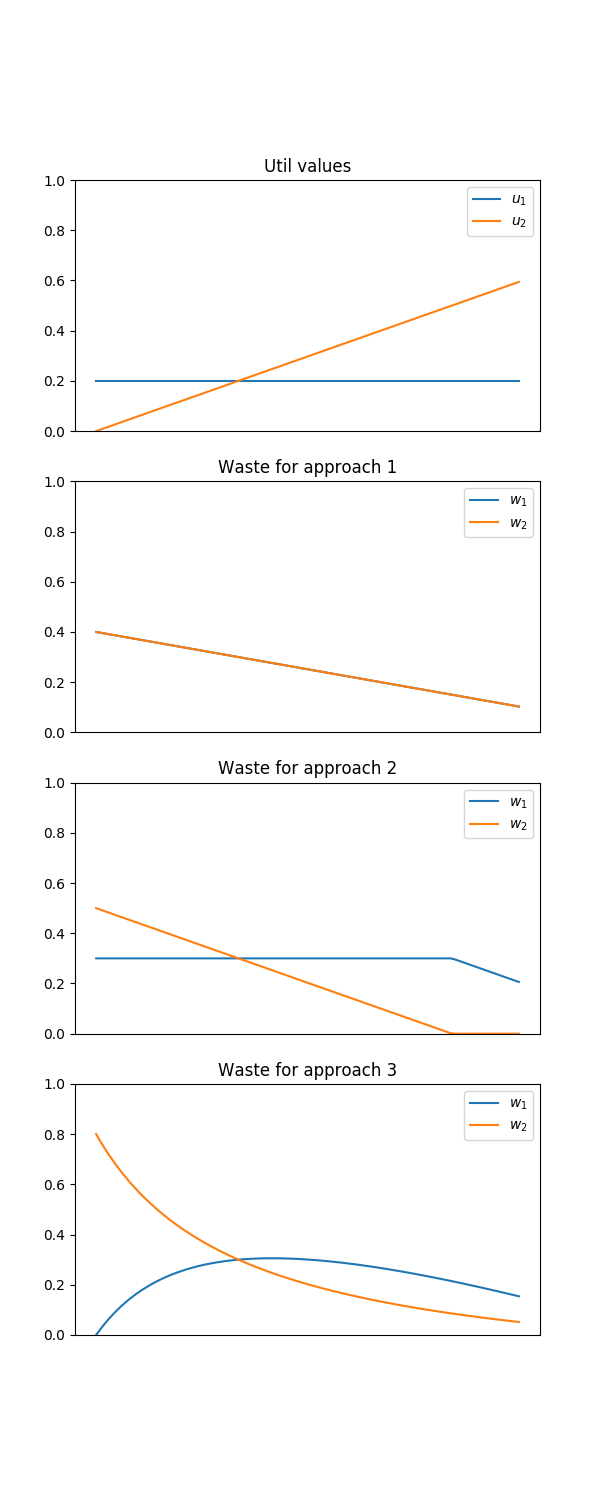
\includegraphics[width=6cm]{gfx/exampleA.png}%
    \label{fig:approaches:A}%
  }\qquad
  \subfloat[Example 2]{%
    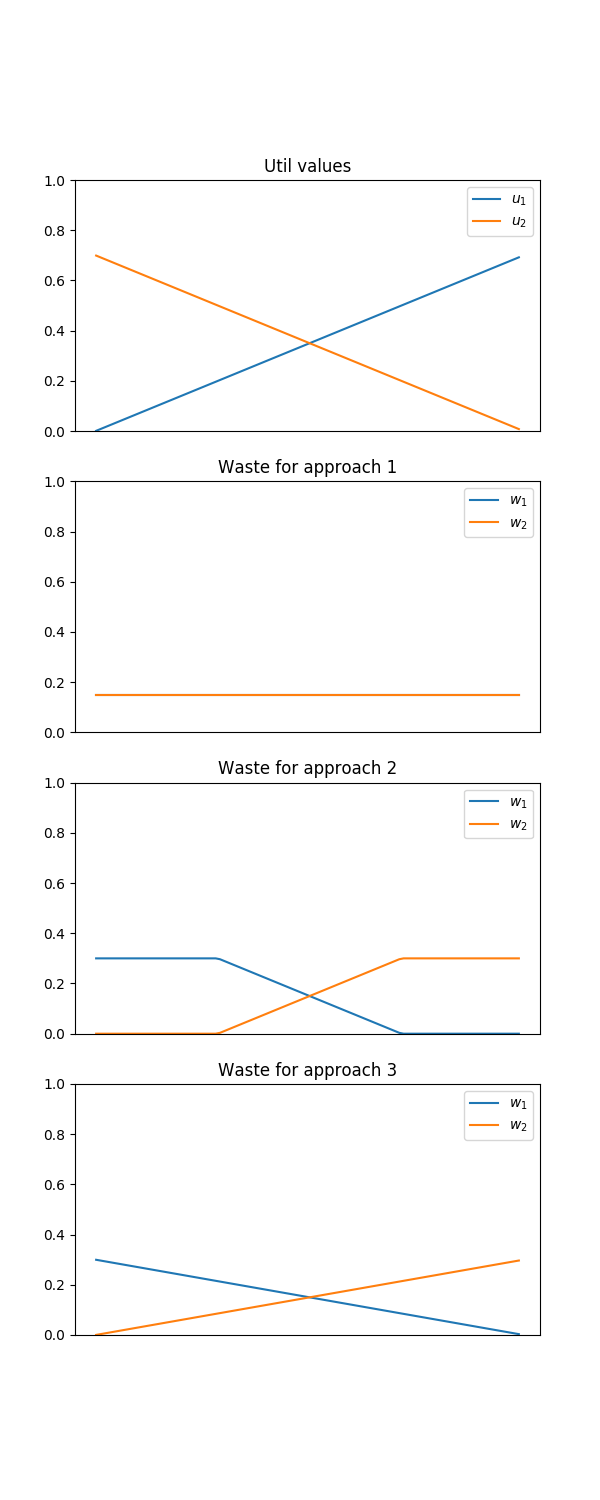
\includegraphics[width=6cm]{gfx/exampleB.png}%
    \label{fig:approaches:B}%
  }
  \caption{Two utilization values and their corresponding waste distribution}
  \label{fig:approaches}
\end{figure}


\section{Conclusion} \label{sec:conclusion4}
One of the properties of the utilization values (as stated in \autoref{sec:utilization}) is that $u_i > 0$ for all $i$. However, while deploying the system, it turned out that the utilization of a certain container was zero. In the first two approaches (\autoref{sec:equal} and \autoref{sec:linear}), this is not a problem. However, this is a problem for the last approach (\autoref{sec:proportional}). An example can be seen for $n = 3$ with $u_1 = 0.3, u_2 = 0, u_3 = 0.2$. This results in the waste values: $w_1 = 0, w_2 = 0.5, w_3 = 0$. Therefore, if $u_1 = 0$, then $w_i = 1 - u$.\\

\noindent
In case there are two containers that have a zero utilization, than the waste cannot be computed for the third approach. This is due to the fact that the matrix $A_n$ does not have a full rank anymore (as two rows are the same). This problem can be avoided by adding a small utilization value $\Delta$ to the $u_i$-values that are $0$. This value can then be removed from the corresponding $w_i$ value, to ensure that property 1 still holds. However, as explained in \autoref{sec:data}, the corresponding $w_i$ will be close to $\sum_{j=1}^n w_j$ and will lead to abnormal results. This leads to the conclusion that only the approach from \autoref{sec:linear} is sufficient for the implementation. Thus, Algorithm \ref{alg:linear} will be used to compute the waste values given the utilization values.